% BDE Guide --- Chapter 2: Popular BDEs for CS Students
\chapter{Popular BDEs for CS Students}
\label{ch:popular-bde}

\begin{quote}
\emph{``Choose BDEs that compound --- not just that are easy.''} Breadth should make you more employable, more literate, and more interesting. Workload matters, but signal matters more.
\end{quote}

\noindent\fbox{\parbox{\dimexpr\linewidth-2\fboxsep-2\fboxrule}{%
\textbf{How to read this chapter.} We list the most-taken BDEs among CS cohorts, grouped by intent (career, language, GPA-management, curiosity), with workload notes and the double-count traps that catch students every semester.}}
\vspace{0.4em}

\section*{Learning Outcomes}
After this chapter you will be able to:
\begin{enumerate}[label=(L\arabic*)]
    \item name 10+ popular BDEs for CS students and what each signals to employers/grad schools;
    \item interpret a BDE workload table (contact hours, assessment mix, group-work load);
    \item identify double-count and exclusion pitfalls (MPE vs.\ BDE, second-major overlap);
    \item apply a 4-question filter to decide whether a candidate BDE is worth your AU.
\end{enumerate}

% ============================================================
\section{Popular BDEs by Intent}
\label{sec:popular-by-intent}

Not every popular BDE is popular for the same reason. Group by \emph{why} you are taking it:

\paragraph{Career-complement (Business / Finance / Analytics).}
CS + business literacy is the most common pairing. Recruiters for SWE, product, and quant-adjacent roles notice it.
\begin{itemize}
    \item \textbf{AB1601 Organisational Behaviour \& Design} (3~AU) --- teams, motivation, org structure; heavy group project + presentation; moderate workload; no prerequisites.
    \item \textbf{AB1202 Statistics \& Analysis} (3~AU) --- overlaps conceptually with SC2000 but coded as Business; check exclusion with SC2000/MH2500 before enrolling.
    \item \textbf{AC1103 Accounting I} / \textbf{BF1101 Finance} --- useful if targeting fintech; quantitative but memorisation-heavy on standards.
    \item \textbf{ET9131 Entrepreneurship I, BM2501 Business Analytics} --- venture/innovation signal; project-heavy.
\end{itemize}

\paragraph{Language BDEs (global mobility).}
NTU's Centre for Modern Languages offers 3--4~AU sequences. CS students over-index here because language + technical skill is rare and durable.
\begin{itemize}
    \item \textbf{LJ5001 Japanese Level~1} (4~AU) $\to$ LJ5002--5006 progression; \textbf{LK5001 Korean}, \textbf{LC5001 Chinese}, \textbf{LF5001 French}, \textbf{LH5001 Hindi} analogous.
    \item 4~AU for Level~1 (more contact hours), then 3~AU for higher levels. Entry by placement test if you have prior knowledge --- do not enrol in Level~1 if you already speak the language; audit will flag it.
\end{itemize}

\paragraph{Human behaviour \& society (HSS / Psychology).}
Design better products, manage teams, understand users.
\begin{itemize}
    \item \textbf{HP1000 Introduction to Psychology} (3~AU) --- perception, memory, social psych; exam + quizzes; no prerequisites; consistently high enrolment.
    \item \textbf{HP8001 Thinking \& Reasoning / HP8101 Mind \& Behaviour} (3~AU) --- lighter, essay-based.
    \item \textbf{HH1001 What Is History? / HAxxxx Art History, HE9091 Principles of Economics} --- HSS breadth; writing-intensive.
\end{itemize}

\paragraph{Science, sustainability \& curiosity.}
\begin{itemize}
    \item \textbf{CM8001 Sustainable Energy, BS8003 Science of Cooking, ES9001 Sustainability} --- popular as ``lighter'' BDEs; check workload --- some have lab components.
    \item \textbf{GC0001 / EE8087 Cyber Ethics or Sustainability-adjacent ICC overflow} --- if not already counting as ICC, may count as BDE; verify with Degree Audit (ICC vs.\ BDE boundary shifts by cohort).
\end{itemize}

\paragraph{Creative \& wellness.}
\begin{itemize}
    \item Photography, film, music, creative writing (various HE/HA/AD codes), and Nanyang Technopreneurship Centre design modules. Workload is often portfolio/project-based --- less exam stress, more time management.
\end{itemize}

% ============================================================
\section{Workload \& Assessment Table}
\label{sec:workload-table}

\begin{table}[h]
\centering
\small
\renewcommand{\arraystretch}{1.22}
\begin{tabular}{@{}p{3.6cm}ccccp{3.1cm}@{}}
\toprule
Course (example) & AU & Contact & Exam & Group & Notes \\
\midrule
HP1000 Intro to Psychology & 3 & 3~h/wk & 40--60\% & Low & Quizzes + exam; no prereq. \\
AB1601 Org.\ Behaviour & 3 & 3~h/wk & 30--40\% & High & Group project + presentation. \\
AB1202 Statistics \& Analysis & 3 & 3~h/wk & 50--60\% & Med & Check exclusion w.\ SC2000. \\
LJ5001 Japanese 1 & 4 & 4~h/wk & 40\% & Low & Daily vocab; placement test if prior. \\
LK5001 Korean 1 & 4 & 4~h/wk & 40\% & Low & Same pattern as LJ. \\
ET9131 Entrepreneurship & 3 & 3~h/wk & 20--30\% & High & Pitch + business plan. \\
CM8001 Sustainable Energy & 3 & 2--3~h/wk & 50\% & Low & Some semesters include lab. \\
HE9091 Economics & 3 & 3~h/wk & 50--60\% & Low & Graph/mechanism heavy. \\
BM2501 Business Analytics & 3 & 3~h/wk & 40\% & Med & Python/R overlap with CS --- easy win. \\
HAxxx / ADxxx (arts/design) & 3 & 2--3~h/wk & 0--20\% & Med & Portfolio-based; time-heavy. \\
\bottomrule
\end{tabular}
\caption{Illustrative workload snapshot for popular BDEs. Exact exam \% and contact hours vary by semester/instructor --- always check the course outline in NTU Course Catalogue before bidding. ``Group'' = group-project load.}
\label{tab:bde-workload}
\end{table}

\begin{remark}[Reading the table]
A ``Low group, 50\% exam'' BDE (HP1000, HE9091) suits a semester already heavy on group-heavy core courses (SC2006, SC3010). A ``High group'' BDE (AB1601, ET9131) is better in a semester with exam-heavy cores. Balance your semester, not just the single course.
\end{remark}

% ============================================================
\section{The Double-Count \& Exclusion Flowchart}
\label{sec:double-count-flow}

The same course cannot satisfy two buckets. Use this decision tree \emph{before} you bid:

\begin{figure}[h]
\centering
\begin{tikzpicture}[scale=0.78,every node/.style={font=\scriptsize},
  decision/.style={diamond,draw,thick,fill=orange!16,aspect=2,align=center,inner sep=2pt},
  action/.style={rectangle,draw,thick,rounded corners=3pt,align=center,inner sep=4pt},
  yes/.style={font=\tiny\bfseries,color=green!55!black},
  no/.style={font=\tiny\bfseries,color=red!65!black}
]
\node[action,fill=blue!10] (start) at (0,3.2) {You want course X};
\node[decision] (q1) at (0,1.85) {Is X in your\\Programme Core?};
\node[action,fill=red!12] (r1) at (5.2,1.85) {Not a BDE.\\(Core already covers it)};
\node[decision] (q2) at (0,0.25) {Is X on your cohort's\\MPE list \& you need MPE?};
\node[action,fill=violet!14] (r2) at (5.2,0.25) {Count as MPE\\(not BDE)};
\node[decision] (q3) at (0,-1.45) {Is X excluded\\w.\ a course you passed?};
\node[action,fill=red!12] (r3) at (5.2,-1.45) {Cannot take\\(exclusion rule)};
\node[decision] (q4) at (0,-3.05) {Does X overlap\\second-major/minor?};
\node[action,fill=green!14] (ok) at (-3.8,-3.05) {Counts as BDE.\\Bid!};
\node[action,fill=yellow!18] (replace) at (3.8,-4.45) {Replaces BDE AU\\(second-major rule)\\--- not extra AU};

\draw[->,thick] (start) -- (q1);
\draw[->,thick] (q1) -- node[yes,above,sloped] {yes} (r1);
\draw[->,thick] (q1) -- node[no,left] {no} (q2);
\draw[->,thick] (q2) -- node[yes,above,sloped] {yes} (r2);
\draw[->,thick] (q2) -- node[no,left] {no} (q3);
\draw[->,thick] (q3) -- node[yes,above,sloped] {yes} (r3);
\draw[->,thick] (q3) -- node[no,left] {no} (q4);
\draw[->,thick] (q4) -- node[no,above,sloped] {no} (ok);
\draw[->,thick] (q4) -- node[yes,above,sloped] {yes} ++(2.8,0) |- (replace);

\node[font=\tiny,align=center,fill=white,inner sep=2pt] at (0,-5.35) {Check exclusions in NTU Course Catalogue; check MPE list for \emph{your cohort year}; confirm in Degree Audit after enrolment.};
\end{tikzpicture}
\caption{Should this course count as BDE? Follow the tree. When in doubt, email your academic advisor \emph{before} bidding --- STARS swaps cost time and may lose your slot.}
\label{fig:bde-flowchart}
\end{figure}

\paragraph{Three concrete traps.}
\begin{enumerate}
    \item \textbf{SC-coded MPE trap.} You take SC4023 (MPE-listed) thinking ``one more SC4xxx as BDE''. It counts as MPE only. If your MPE bucket is already full (9 courses + FYP), the extra SC4xxx may still count as BDE --- but only if you \emph{declare} it unused for MPE and your Degree Audit agrees. Do not assume; declare explicitly.
    \item \textbf{AB1202 $\leftrightarrow$ SC2000 exclusion.} Some Business statistics courses exclude SC2000/MH2500. You passed SC2000 in Y1. AB1202 may be blocked. Check the ``Mutually exclusive'' line in the catalogue, not just prerequisites.
    \item \textbf{Language placement.} You speak conversational Korean and enrol in LK5001 (Beginner). The Centre for Modern Languages may require a placement test and reassign you to LK5003. Taking LK5001 anyway risks AU not counting.
\end{enumerate}

% ============================================================
\section{A 4-Question Filter for Any Candidate BDE}
\label{sec:bde-filter}

Before you bid, score the candidate 1--5 on each:

\begin{center}
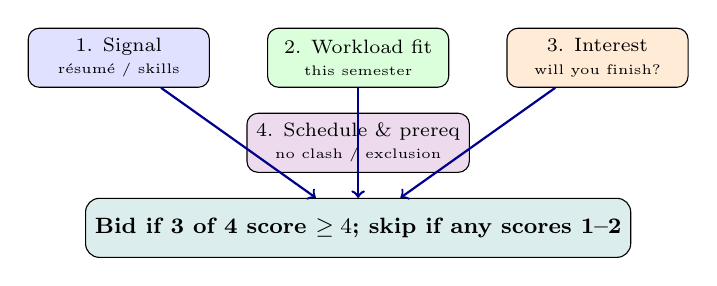
\begin{tikzpicture}[scale=0.80,every node/.style={font=\scriptsize}]
\node[draw,fill=blue!12,rounded corners=4pt,minimum width=2.3cm,minimum height=0.75cm,align=center] (q1) at (-3.8,1.0) {1. Signal\\{\tiny r\'esum\'e / skills}};
\node[draw,fill=green!14,rounded corners=4pt,minimum width=2.3cm,minimum height=0.75cm,align=center] (q2) at (0,1.0) {2. Workload fit\\{\tiny this semester}};
\node[draw,fill=orange!16,rounded corners=4pt,minimum width=2.3cm,minimum height=0.75cm,align=center] (q3) at (3.8,1.0) {3. Interest\\{\tiny will you finish?}};
\node[draw,fill=violet!14,rounded corners=4pt,minimum width=2.5cm,minimum height=0.75cm,align=center] (q4) at (0,-0.35) {4. Schedule \& prereq\\{\tiny no clash / exclusion}};
\node[draw,fill=teal!14,rounded corners=5pt,minimum width=5.5cm,minimum height=0.75cm,align=center,font=\footnotesize\bfseries] (out) at (0,-1.7) {Bid if 3 of 4 score $\ge 4$; skip if any scores 1--2};
\foreach \target in {q1,q2,q3} \draw[->,thick,blue!55!black] (\target) -- (out);
\draw[->,thick,blue!55!black] (q4) -- (out);
\end{tikzpicture}
\end{center}

A BDE that scores 5 on interest but 1 on workload fit for \emph{this} semester should wait --- the catalogue repeats most BDEs every semester or year.

% ============================================================
\section{Chapter Notes}
Course examples and workload patterns synthesised from NTU Course Catalogue entries, NTUMods, and CCDS student forum reports at time of writing; offerings, AUs, and assessment mixes vary by semester and instructor. Always verify prerequisites, exclusions, and MPE-list status for your cohort year before bidding.

% ============================================================
\section{Exercises}
\label{sec:ch02-exercises}
\begin{enumerate}[label=E2.\arabic*, leftmargin=*, itemsep=0.8em]
    \item \textbf{Workload balancing.} You are taking SC2006 (group-heavy) + SC2005 (exam-heavy) + SC2203 (proof-heavy) in one semester and want one BDE. Which BDE from Table~\ref{tab:bde-workload} balances best, and why?
    \item \textbf{Exclusion check.} You passed SC2000. A friend says AB1202 is a free 3~AU BDE. What do you check before bidding, and where?
    \item \textbf{MPE vs.\ BDE declaration.} You have 8 MPE courses done and need one more MPE at 4000-level. You also want SC4023 as a BDE. Can SC4023 satisfy both? What must you do in Degree Audit if your MPE bucket is already full?
    \item \textbf{Language placement.} You grew up speaking Japanese at home. Should you enrol in LJ5001? What is the correct first step?
\end{enumerate}
% End of Chapter 2
